\documentclass[12pt,a4paper,utf8x]{report}
\usepackage [francais]{babel}
\usepackage[utf8]{inputenc}  
\usepackage[T1]{fontenc} 
% Pour pouvoir utiliser 
\usepackage{ucs}
\usepackage{textcomp}
\usepackage{graphicx}
\usepackage{keystroke}
\usepackage{amssymb}
\usepackage{amsmath}
%\usepackage{pifont}
\usepackage{url} % Pour avoir de belles url
\usepackage{geometry}
\usepackage{hyperref}


\usepackage {listings}% Pour mettre du code source
\lstset{language=sh}

% Pour pouvoir passer en paysage
\usepackage{lscape}

% Pour pouvoir faire plusieurs colonnes
\usepackage {multicol}

\usepackage{makeidx}% Pour crééer un index
\usepackage{graphicx} % Pour insérer des images (entres autres)
\usepackage{fourier-orns} %logo comme \danger
\usepackage[cc]{titlepic} %rajouter le logo 	 dans la page de garde
\usepackage{tocbibind}
%\usepackage{wasysym} %emoticones
\usepackage{glossaries} % Créer un glossaire
\hypersetup{
  backref=true,
  %permet d'ajouter des liens dans...
  pagebackref=true,%...les bibliographies
  hyperindex=true, %ajoute des liens dans les index.
  colorlinks=true, %colorise les liens
  breaklinks=true, %permet le retour à la ligne dans les liens trop longs
  urlcolor= blue, %couleur des hyperliens
  bookmarks=true, %créé des signets pour Acrobat
  bookmarksopen=true,
  %si les signets Acrobat sont créés,
  %les afficher complètement.
  pdftitle={Eclipse Vision System Plugin}, %informations apparaissant dans
  pdfauthor={MARGUERITE Alain\\ RINCE Romain},
  %dans les informations du document
  pdfsubject={LoCD}
  %sous Acrobat.
}
%Entête pied de page
%Définition des entêtes : 
\usepackage{fancyhdr}
\pagestyle{fancy}

\lstset{language=XML,    numbers=left
   , tabsize=2
   , frame=single
   , breaklines=true
   , basicstyle=\ttfamily
   , numberstyle=\tiny\ttfamily
   , framexleftmargin=13mm
   , xleftmargin=12mm
   %, frameround={tttt}
   , captionpos=b  }
%\usepackage{pifont}
\usepackage[cc]{titlepic}
\usepackage{url} % Pour avoir de belles url
\usepackage {geometry}

% Pour mettre du code source
\usepackage {listings}
% Pour pouvoir passer en paysage
\usepackage{lscape}

% Pour pouvoir faire plusieurs colonnes
\usepackage {multicol}
% POur crééer un index
\usepackage{makeidx}
\usepackage{graphicx}
\makeindex

% Pour l'interligne de 1.5
\usepackage {setspace}
% Pour les marges de la page
\geometry{a4paper, top=2.5cm, bottom=3.5cm, left=1.5cm, right=1.5cm, marginparwidth=1.2cm}

\parskip=5pt %% distance entre § (paragraphe)
\sloppy %% respecter toujours la marge de droite 

% Pour les pénalités :
\interfootnotelinepenalty=150 %note de bas de page
\widowpenalty=150 %% veuves et orphelines
\clubpenalty=150 

%Pour la longueur de l'indentation des paragraphes
\setlength{\parindent}{15mm}



%%%% debut macro pour enlever le nom chapitre %%%%
\makeatletter
\def\@makechapterhead#1{%
  \vspace*{50\p@}%
  {\parindent \z@ \raggedright \normalfont
    \interlinepenalty\@M
    \ifnum \c@secnumdepth >\m@ne
        \Huge\bfseries \thechapter\quad
    \fi
    \Huge \bfseries #1\par\nobreak
    \vskip 40\p@
  }}

\def\@makeschapterhead#1{%
  \vspace*{50\p@}%
  {\parindent \z@ \raggedright
    \normalfont
    \interlinepenalty\@M
    \Huge \bfseries  #1\par\nobreak
    \vskip 40\p@
  }}
\makeatother
%%%% fin macro %%%%

%Couverture 



\title
{
	\normalsize{ M1 ALMA\\ 
	Université de Nantes\\
	2011-2012}\\
	\vspace{15mm}
	\Huge{Projet de Travaux pratiques :\\TOA \\ Eclipse Vision System Plugin}
}



\author{BIZET Jonathan\\CHALIN Jeremy\\ MARGUERITE Alain\\ RINCÉ Romain 
	\vspace{45mm}
}
\titlepic{
\includegraphics[scale=1.00]{img/logouniv}   }
\date
{	
	\normalsize{Université de Nantes \\ 2 rue de la Houssinière, BP92208, F-44322 Nantes cedex 03, FRANCE
	\\ 
	\vspace{5mm}	
	Encadrant : Gilles Ardourel, Dalila Goudia, Sagar Sen
\\
	}
}

\begin{document}
\renewcommand{\labelitemi}{$\bullet$} 	
\maketitle


\clearpage

\tableofcontents
\clearpage

% Pour avoir un interligne de 1,5
\begin{onehalfspace}
\chapter{Introduction}
   \begin{figure}[htbp]
  \centering
  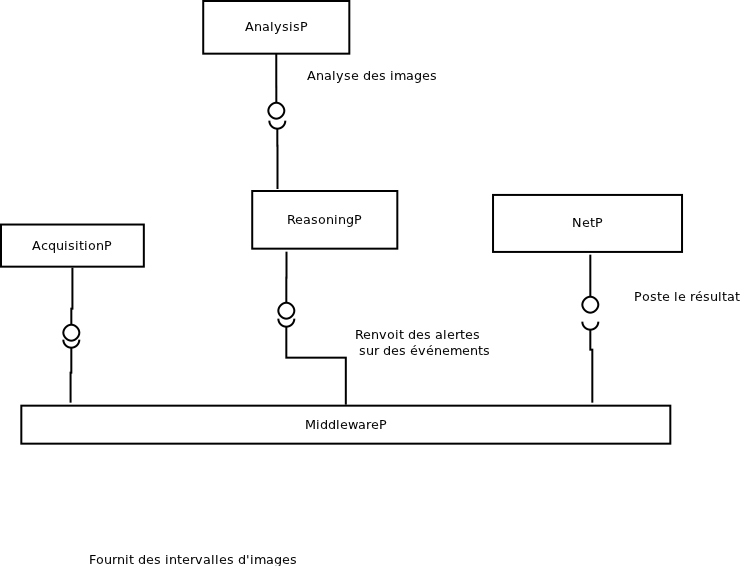
\includegraphics[scale=0.70]{img/archi}
  \caption{Architecture de l'outil}
  \label{fig:archi}
\end{figure}

\chapter{Architecture}
Dans cette partie nous détaillerons l'architecture de notre application, à travers ses différents points d'extensions.
\begin{figure}[htbp]
  \centering
  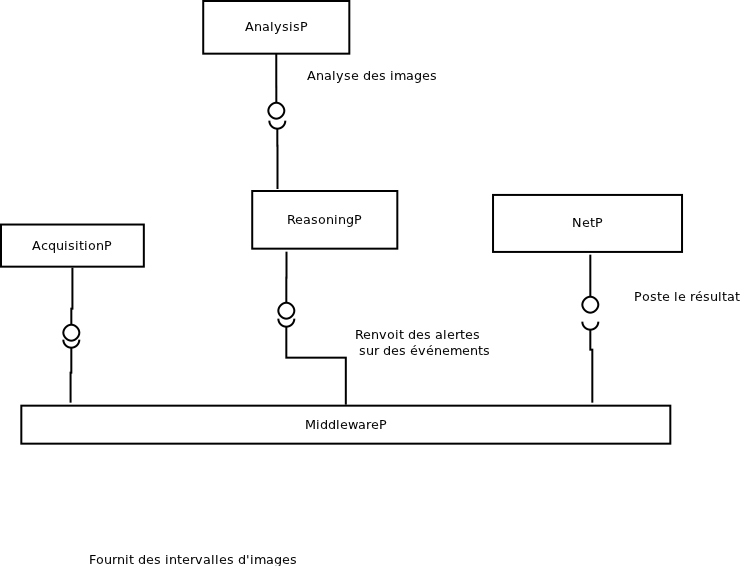
\includegraphics[scale=0.70]{img/archi}
  \caption{Architecture de l'outil}
  \label{fig:archi}
\end{figure}

\section{Acquisition}
Le plugin Acquisition consiste à récupérer un fichier vidéo et en extraire une image périodiquement. Le plugin répond aux spécifications fournies par l'interface \verb+IFlux+ (cf. Fig \ref{})
\begin{figure}[htbp]
  \centering
  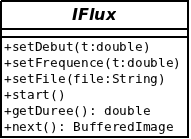
\includegraphics[scale=0.50]{img/IFlux}
  \caption{Interface IFlux}
  \label{fig:IFlux}
\end{figure}
\section{Reasoning}

\section{NetP}
Le  NetP est dédié à poster des informations sur un  réseau social ou un blog. Un contributeur de ce point d'extension doit être en mesure de proposer une solution pour chaque action que recquière Middleware. Ces actions sont données dans l'interface \verb+IIformation+ suivante :
\begin{figure}[htbp]
  \centering
  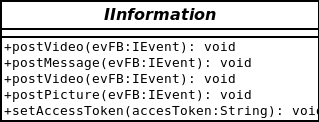
\includegraphics[scale=0.50]{img/iinterface}
  \caption{Interface pour NetP}
  \label{fig:IInterface}
\end{figure}

Le contributeur que nous avons implémenté propose d'utiliser le réseau social Facebook et utilise la librairie suivante \cite{restFB}.






\chapter{Documentation}



% Pour finir l'interligne de 1,5
\end{onehalfspace}



\listoffigures

\printindex

\appendix

\bibliographystyle{alpha}
\bibliography{biblio.bib}


\end{document}
